% !TeX program = xelatex
\documentclass[12pt,aspectratio=169]{beamer}
\usepackage[UTF8,fontset=fandol]{ctex}
\usepackage{amsmath,booktabs,graphicx,array}
\usepackage{pdfbase}
% Native H.264 RichMedia, without a Flash player.
% Uses the installed pdfbase driver API and the PDF RichMedia object model.
\ExplSyntaxOn
\box_new:N \l_defense_poster_box
\NewDocumentCommand \embeddefensevideo {mm} {
  \group_begin:
  \leavevmode
  \pbs_pdfobj:nnn {} {fstream}
    {{/Type/EmbeddedFile/Subtype/video\c_hash_str 2Fmp4}{#2}}
  \pbs_pdfobj:nnn {} {dict} {
    /Type/Filespec/F~(demo.mp4)/UF~(demo.mp4)
    /EF~<</F~\pbs_pdflastobj:>>
  }
  \tl_set:Nx \l_defense_asset_tl {\pbs_pdflastobj:}
  \pbs_pdfobj:nnn {} {dict} {
    /Type/RichMediaInstance/Subtype/Video/Asset~\l_defense_asset_tl
  }
  \pbs_pdfobj:nnn {} {dict} {
    /Type/RichMediaConfiguration/Subtype/Video/Instances~[\pbs_pdflastobj:]
  }
  \tl_set:Nx \l_defense_config_tl {\pbs_pdflastobj:}
  \pbs_pdfobj:nnn {} {dict} {
    /Type/RichMediaContent
    /Assets~<</Names~[(demo.mp4)~\l_defense_asset_tl]>>
    /Configurations~[\l_defense_config_tl]
  }
  \tl_set:Nx \l_defense_content_tl {\pbs_pdflastobj:}
  \pbs_pdfobj:nnn {} {dict} {
    /Type/RichMediaSettings
    /Activation~<</Condition/XA/Configuration~\l_defense_config_tl
      /Presentation~<</Style/Embedded/Toolbar~true/PassContextClick~true>>>>
    /Deactivation~<</Condition/PI>>
  }
  \tl_set:Nx \l_defense_settings_tl {\pbs_pdflastobj:}
  \hbox_set:Nn \l_defense_poster_box {#1}
  \pbs_pdfxform:nnnnn {1}{1}{}{}{\l_defense_poster_box}
  \pbs_pdfannot:nnnn
    {\box_wd:N\l_defense_poster_box}
    {\box_ht:N\l_defense_poster_box}
    {\box_dp:N\l_defense_poster_box} {
      /Subtype/RichMedia/F~4/BS~<</W~0>>
      /Contents~(Click~to~play~the~embedded~demonstration~video)
      /NM~(defense-demo-video)
      /AP~<</N~\pbs_pdflastxform:>>
      /RichMediaContent~\l_defense_content_tl
      /RichMediaSettings~\l_defense_settings_tl
    }
  \box_use:N \l_defense_poster_box
  \group_end:
}
\pbs_pdfcatalog:n {/Extensions~<</ADBE~<</BaseVersion/1.7/ExtensionLevel~3>>>>}
\ExplSyntaxOff

\usefonttheme{professionalfonts}
\setbeamertemplate{navigation symbols}{}
\definecolor{Ink}{HTML}{172B3A}
\definecolor{Teal}{HTML}{087F8C}
\definecolor{Muted}{HTML}{5C6E78}
\definecolor{Pale}{HTML}{D8EDF0}
\setbeamercolor{normal text}{fg=Ink,bg=white}
\setbeamercolor{structure}{fg=Teal}
\setbeamercolor{frametitle}{fg=Ink}
\setbeamerfont{frametitle}{size=\fontsize{23}{28}\selectfont,series=\bfseries}
\setbeamersize{text margin left=8mm,text margin right=8mm}
\setbeamertemplate{frametitle}{\vspace{3mm}\centering\insertframetitle\par\vspace{2mm}}
\setbeamertemplate{itemize item}{\raisebox{.15ex}{\scriptsize$\bullet$}}
\setlength{\parskip}{1.5pt}
\setbeamertemplate{footline}{%
  \hbox{\begin{beamercolorbox}[wd=\paperwidth,ht=3mm,dp=3mm,rightskip=8mm]{normal text}%
    \hfill{\color{Muted}\fontsize{8}{10}\selectfont\insertframenumber\,/\,\inserttotalframenumber}%
  \end{beamercolorbox}}}
\newcommand{\lead}[1]{{\color{Teal}\bfseries #1}}
% Supplementary captions are retained in the source for reference, but omitted from slides.
\newcommand{\source}[1]{}
\newcommand{\keyline}[1]{\par\vspace{3mm}{\centering\color{Teal}\fontsize{15}{19}\selectfont\bfseries #1\par}}
% Replace these two fields before the defense.
\newcommand{\presenter}{指导老师：徐鹏}
\newcommand{\affiliation}{团队成员：刘一为、洪驰、李承烨、郑嘉沣}
\hypersetup{colorlinks=true,urlcolor=Teal,pdftitle={To See Is To Touch：视觉触觉三维形状重建},pdfauthor={项目答辩}}
\ifdefined\defensenotes
  \setbeameroption{show only notes}
\else
  \setbeameroption{hide notes}
\fi

\begin{document}

  % 01 / 00:00--00:10
  {\setbeamercolor{background canvas}{bg=Ink}
    \setbeamertemplate{footline}{}
    \begin{frame}[plain]
      \centering
      \vspace*{7mm}
      {\color{Pale}\fontsize{16}{20}\selectfont To See Is To Touch\par}
      \vspace{6mm}
      {\color{white}\fontsize{29}{36}\selectfont\bfseries 机器人触觉传感器\par}
      \vspace{4mm}
      {\color{Pale}\fontsize{14}{19}\selectfont 从接触引起的光学变化，恢复表面几何\par}
      \vspace{11mm}
      {\color{white}\fontsize{10}{15}\selectfont\presenter\par
        \vspace{1mm}\affiliation\par}
      \vspace*{4mm}
      \note{【10 秒，累计 00:10】各位老师好，我们的项目是“视觉触觉三维形状重建”。我们希望让相机看到接触造成的形变，再把这种变化恢复成三维表面。}
  \end{frame}}

  % 02 / 00:10--00:35
  \begin{frame}[c]{从接触形变到视觉信号}
    \begin{columns}[c,onlytextwidth]
      \column{.59\textwidth}
        \centering
        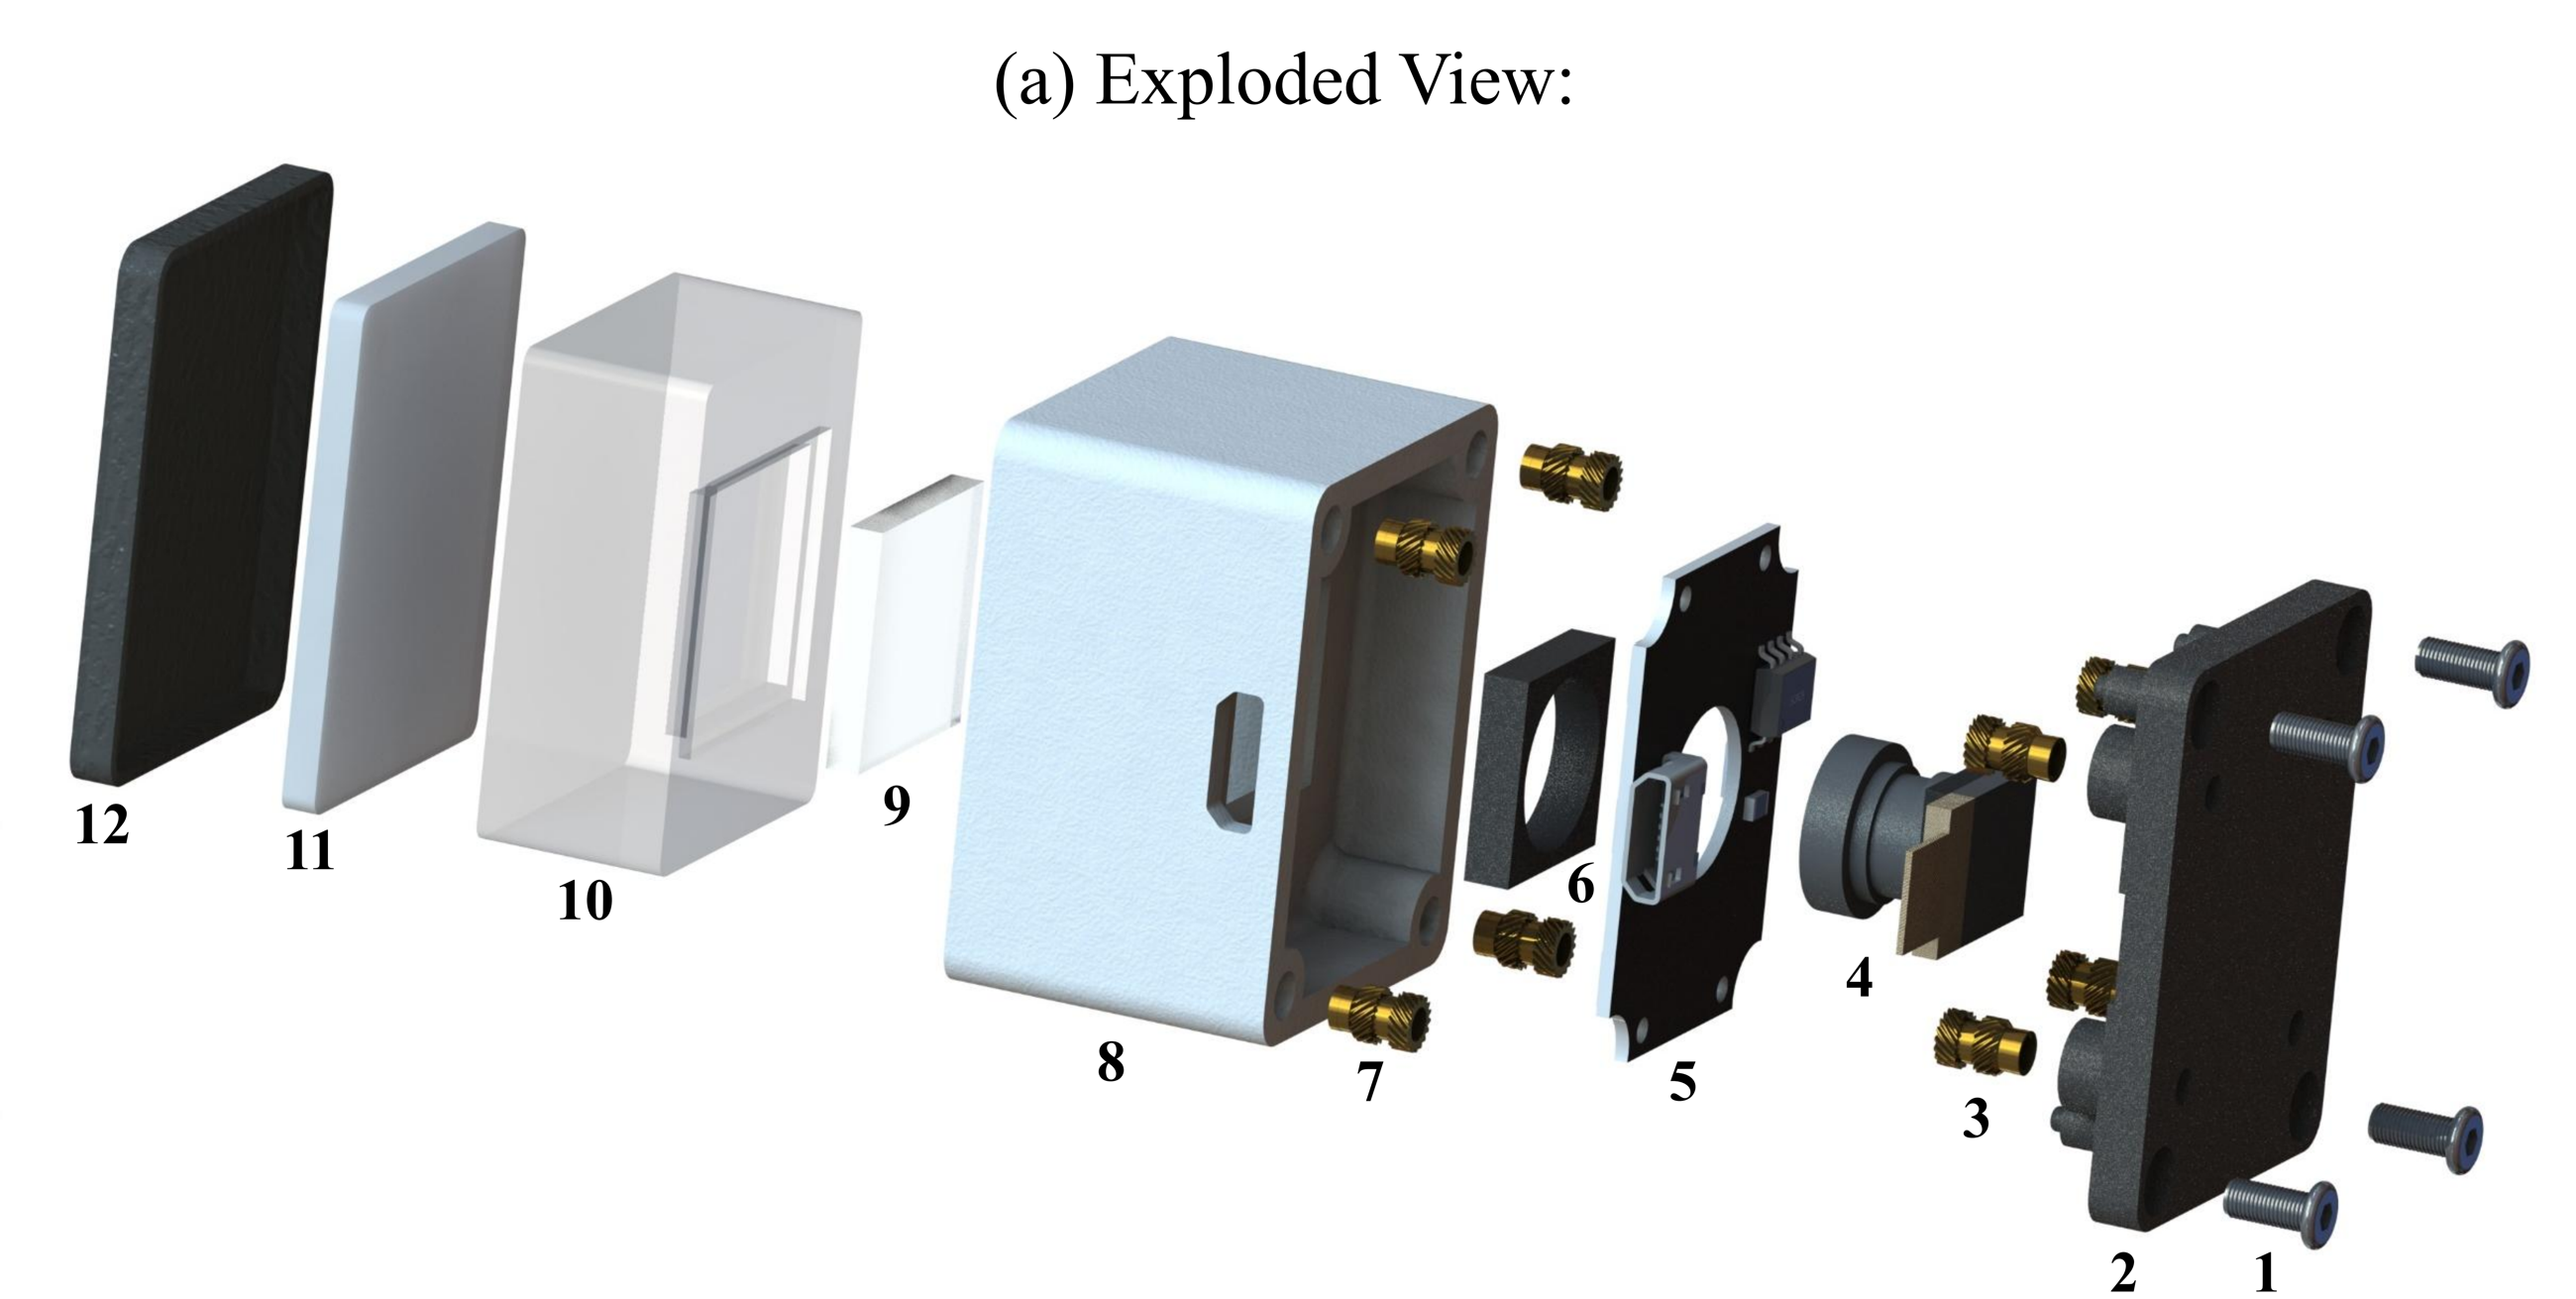
\includegraphics[width=\linewidth,height=38mm,keepaspectratio]{images/design_exploded.png}
      \column{.37\textwidth}
        \lead{接触层}\par 黑色层与半透明凝胶\par
        \vspace{2mm}
        \lead{光学层}\par 白光 LED 与光路约束\par
        \vspace{2mm}
        \lead{采集层}\par 记录接触灰度变化\par
    \end{columns}
    \vspace{2mm}
    \keyline{我们基于 9DTact 的机械结构开发}
    {\centering\small 围绕相机标定、形状重建与实时展示，搭建完整处理流程\par}
    \note{【25 秒，累计 00:35】我们基于 9DTact 的机械结构开发。结构可以分成三部分：上面是接触物体的凝胶，中间是照明和光路，下面是相机。物体压在表面时，凝胶会形变，内部相机记录到相应的灰度变化。本项目围绕标定、重建与实时展示，搭建从图像到几何的完整流程。}
  \end{frame}

  % 03 / 00:35--01:20
  \begin{frame}[c]{为什么压得越深，图像越暗？}
    \begin{columns}[c,onlytextwidth]
      \column{.59\textwidth}
        \centering
        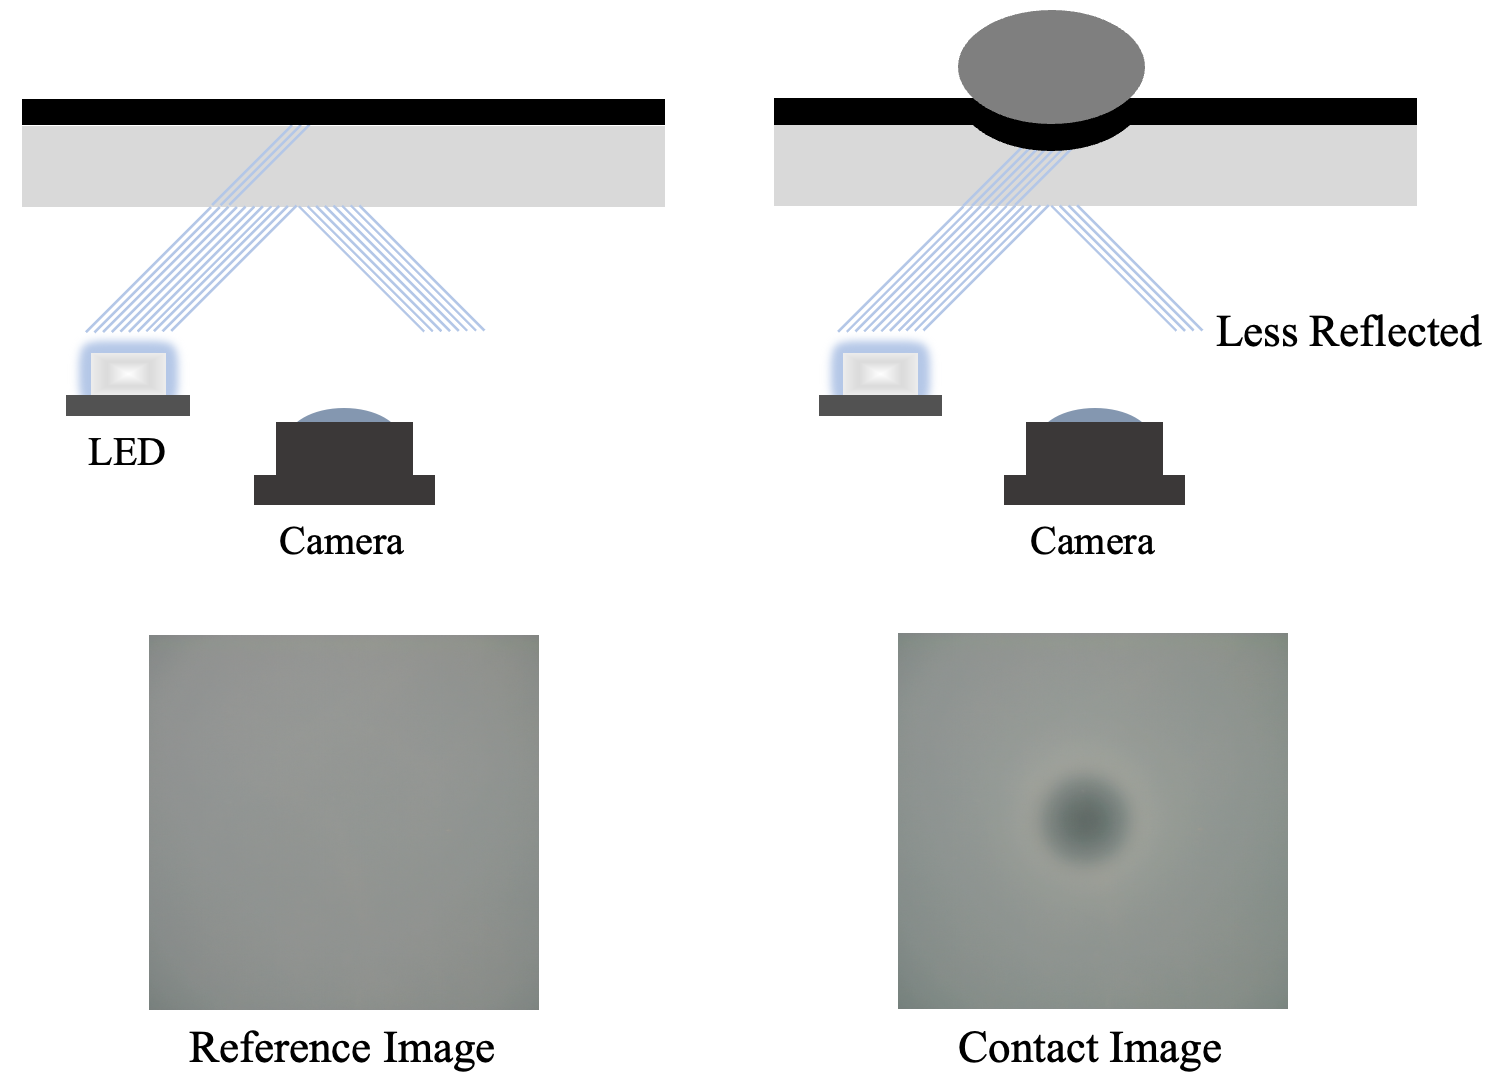
\includegraphics[width=\linewidth,height=43mm,keepaspectratio]{images/optical_principle.png}
        \source{光学原理：裁切保留空载与接触状态}
      \column{.37\textwidth}
        \lead{1\quad 材料决定光学响应}\par
        {\small 黑色硅胶吸光；半透明硅胶反射、散射光。\par}
        \vspace{2mm}
        \lead{2\quad 接触改变凝胶厚度}\par
        {\small 受压区域变薄，返回相机的光减少。\par}
        \vspace{2mm}
        \lead{3\quad 灰度差表征压入量}\par
        {\small 在标定条件与量程内，变暗程度可映射到深度。\par}
    \end{columns}
    \vspace{2mm}
    {\centering\small 用空载参考做差，提取接触引起的变化\par}
    \note{【45 秒，累计 01:20】关键是两种硅胶的光学性质不同。黑色表层吸收光，半透明凝胶会反射和散射光。没有接触时，凝胶较厚，返回相机的光相对较多；受到按压后，局部凝胶变薄，返回的光减少，因此接触区域变暗。我们用空载参考图减去接触图，得到灰度差。越明显的变暗，通常对应越大的压入深度。但灰度本身没有毫米单位，而且受到光照和材料影响，所以还需要标定，不能直接把灰度当作距离。}
  \end{frame}

  % 04 / 01:20--02:05
  \begin{frame}[c]{两步标定，建立毫米尺度}
    \begin{columns}[T,onlytextwidth]
      \column{.49\textwidth}
        \lead{第一步：几何标定}\par
        {\small 用规则点阵校正畸变，确定像素尺度 \(s\)。\par}
        \vspace{1mm}
        \makebox[\linewidth][c]{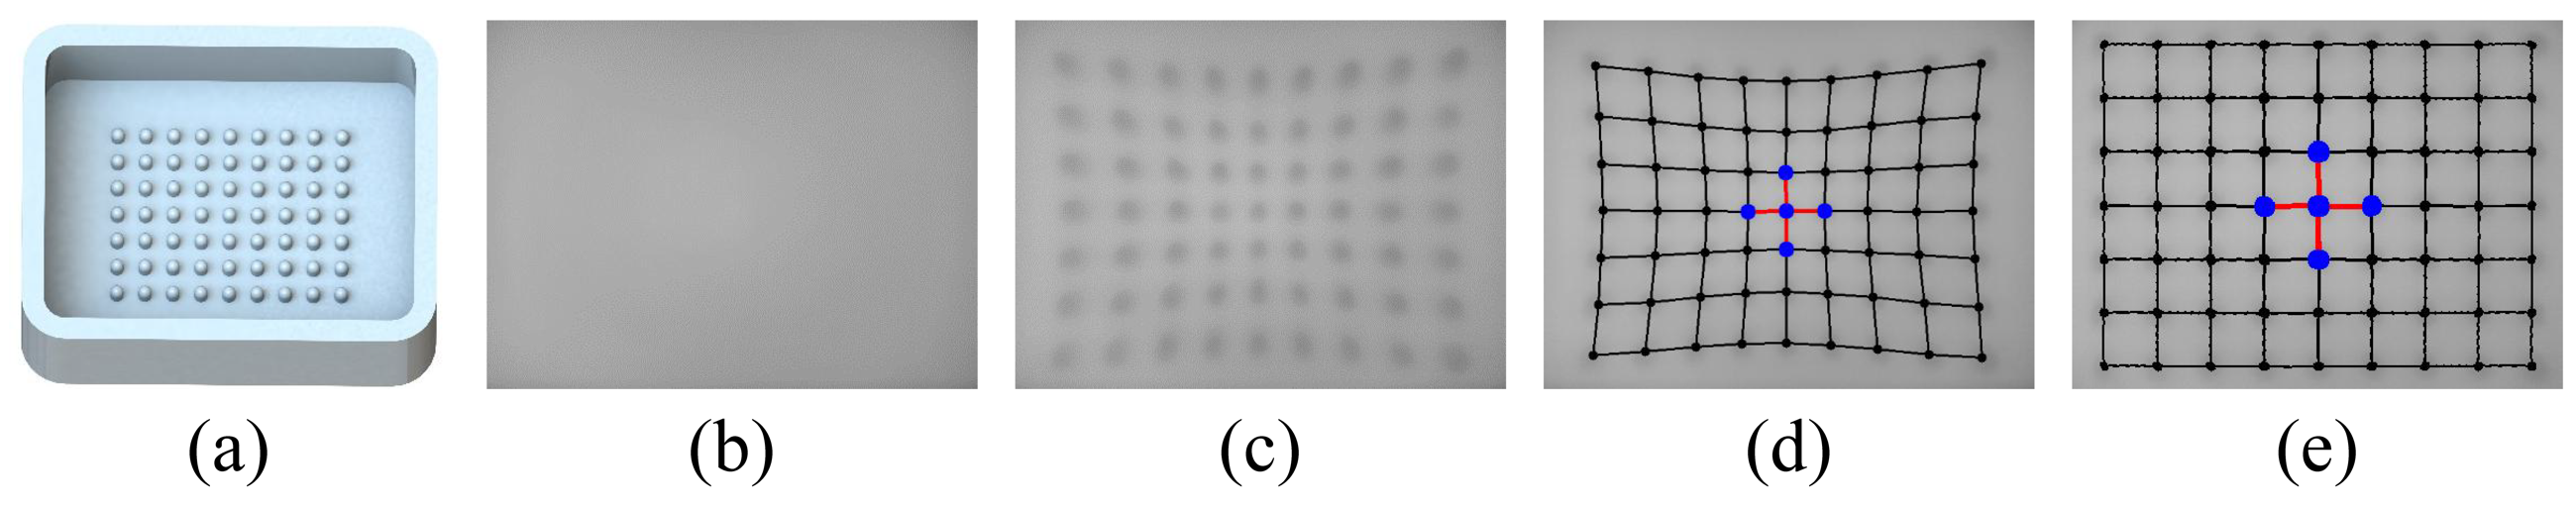
\includegraphics[width=\linewidth,height=24mm,keepaspectratio]{images/calibration.png}}
        \source{点阵、原图与矫正结果。}
        {\small \(s\) 的单位为 mm/pixel\par
          当前配置：点阵间距 \(3\,\mathrm{mm}\)，裁剪 \(300\times400\)。}
      \column{.47\textwidth}
        \lead{第二步：深度标定}\par
        {\small 用已知半径的球接触凝胶。\par}
        \vspace{1mm}
        \centering
        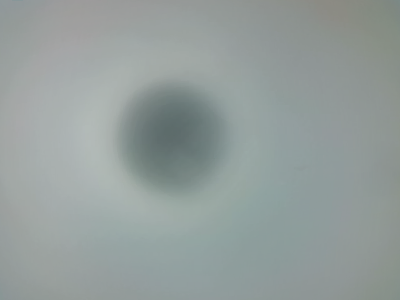
\includegraphics[height=25mm]{images/ball_calibration.png}
        \par\raggedright
        {\small 球面几何给出深度 \(h\)，与灰度差 \(D\) 配对，建立查找表 \(h=f(D)\)。}
        \source{项目保存的球接触标定图；配置球半径 \(R=4\,\mathrm{mm}\)。}
    \end{columns}
    \keyline{先知道“一个像素多长”，再知道“变暗对应多深”。}
    \note{【45 秒，累计 02:05】标定分两步。第一步解决平面位置：用间距已知的规则点阵校正镜头畸变，确定一个像素对应多少毫米。当前配置采用三毫米点阵间距，最终裁剪为三百乘四百。第二步解决深度：用已知半径的球按压，球面几何能够给出接触区域各位置的压入量；再把这些深度与对应的灰度差配对，建立查找表。这样横向位置和纵向深度就都具有物理尺度了。}
  \end{frame}

  % 05 / 02:05--02:40
  \begin{frame}[c]{从二维图像恢复三维表面}
    \centering
    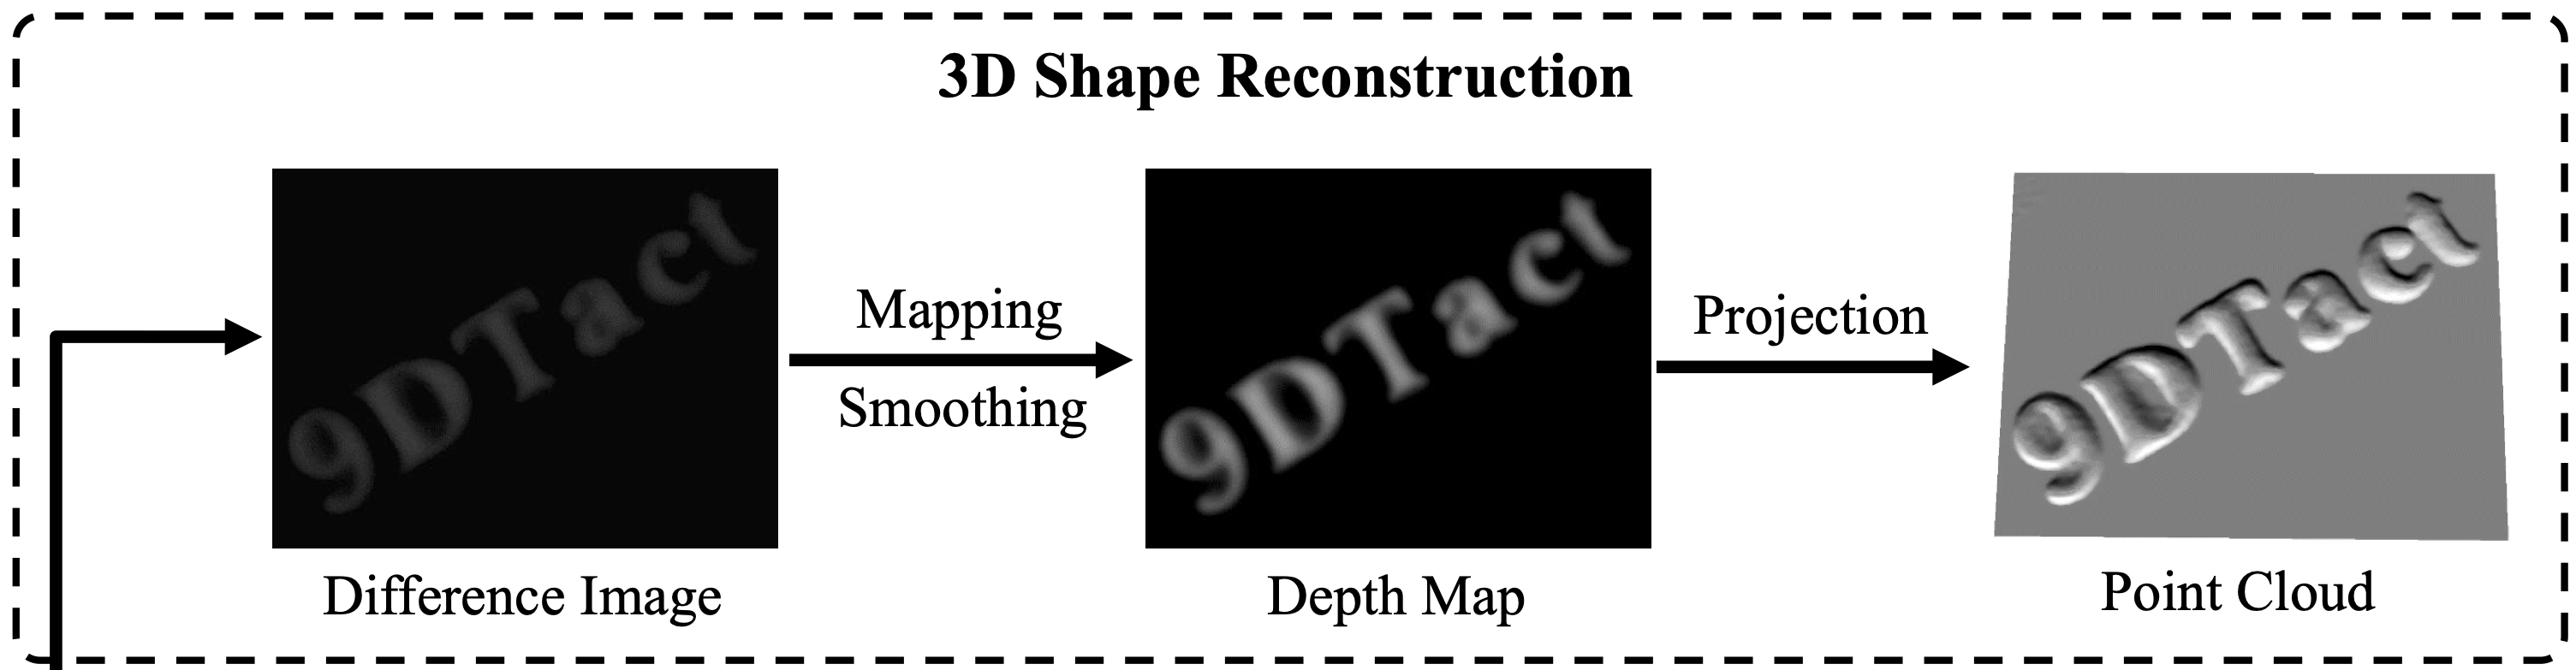
\includegraphics[width=.94\linewidth,height=27mm,keepaspectratio]{images/reconstruction_flow.png}
    \source{9DTact 原项目重建流程示意，仅节选三维形状分支；图中示例非本项目实验结果。}
    \vspace{1mm}
    \begin{columns}[c,onlytextwidth]
      \column{.50\textwidth}
        \raggedright
        \lead{传统重建路径}\par
        {\small 矫正／裁剪 \(\rightarrow\) 参考差分\par
          噪声抑制 \(\rightarrow\) 查表映射 \(\rightarrow\) 平滑高度图}
      \column{.46\textwidth}
        \raggedright
        \lead{点云坐标}\par
        \(\mathbf p(u,v)=\bigl(su,-sv,h(u,v)\bigr)\)\par
        {\small 每个像素对应一个三维点。\par}
    \end{columns}
    \keyline{恢复的是接触区域的表面形变。}
    \note{【35 秒，累计 02:40】得到标定后，每一帧先做矫正、裁剪和参考差分，再抑制噪声，通过查表把灰度变化转换成高度，最后平滑表面。将像素坐标乘以毫米尺度，再把高度放到第三个坐标，就得到点云。这里正方向表示压入深度，显示时可以把它画成凸起。它表达的是接触区域的表面形变，不能直接恢复物体未接触的部分。}
  \end{frame}

  % 06 / 02:40--03:00
  \begin{frame}[c]{训练数据如何构建}
    \begin{columns}[c,onlytextwidth]
      \column{.66\textwidth}
        \centering
        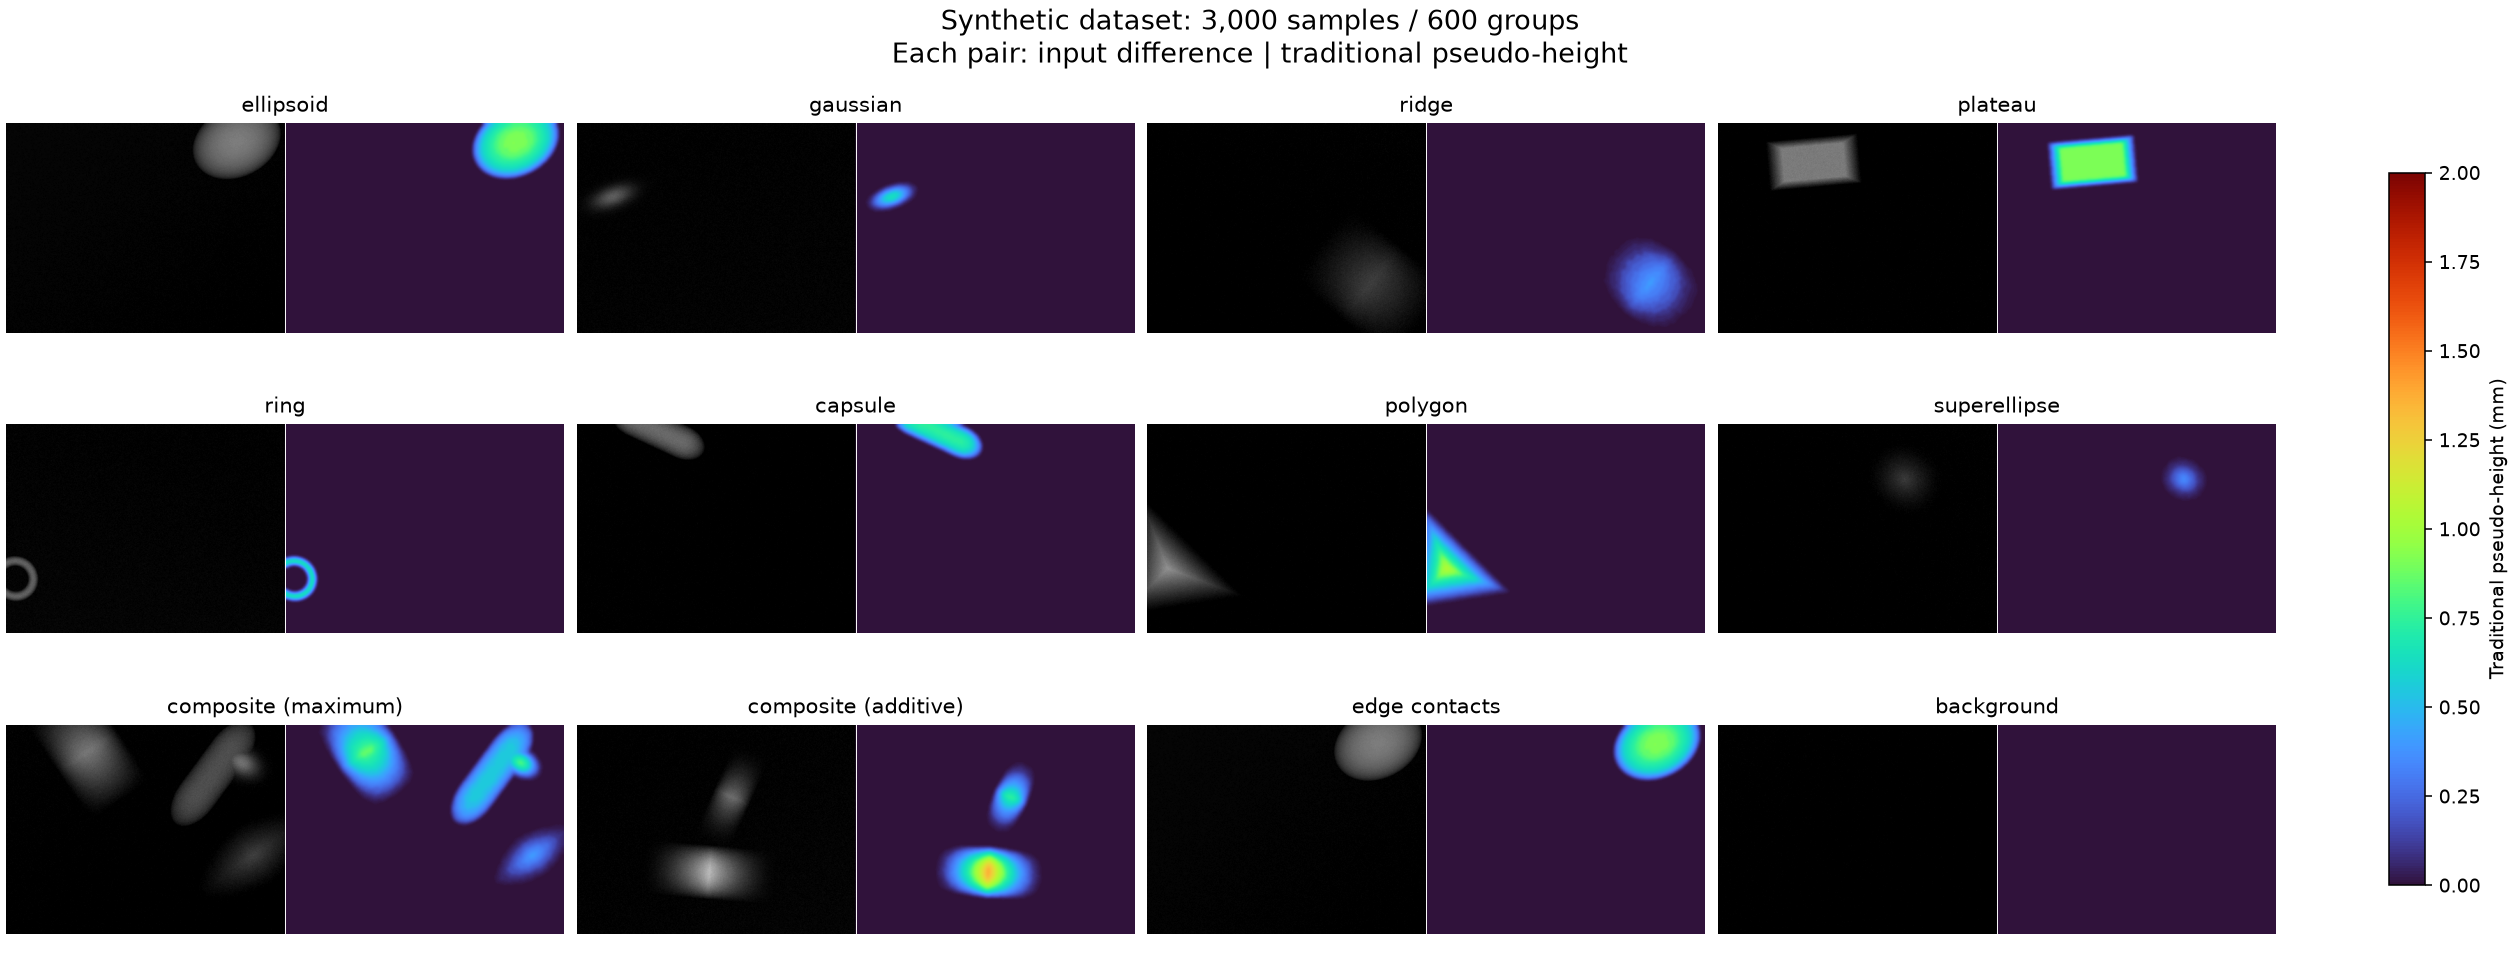
\includegraphics[width=\linewidth]{images/training_diversity.png}
      \column{.30\textwidth}
        \lead{形状多样}\par
        {\small 8 类基本形状\par 圆顶、棱脊、圆环等\par}
        \vspace{2mm}
        \lead{接触多样}\par
        {\small 单点、多点组合\par 边缘接触与空载背景\par}
        \vspace{2mm}
        \lead{条件多样}\par
        {\small 位置、尺寸、方向\par 光照、纹理与噪声\par}
    \end{columns}
    \keyline{3,000 帧合成数据，覆盖 600 个接触组}
    \vspace{1mm}
    {\centering\small 合成接触图像，使用传统算法生成高度伪标签\par}
    \note{【20 秒，累计 03:00】现阶段缺少独立深度测量硬件，我们采用合成图像与传统算法伪标签构建训练集。数据覆盖八类基本形状，以及多点组合、边缘接触和空载背景，并改变位置、尺寸、方向、光照、纹理和噪声。目前共三千帧、六百个接触组。}
  \end{frame}

  % 07 / 03:00--03:40
  \begin{frame}[c]{网络如何学习“灰度差到高度”？}
    \vspace{-1mm}
    \[
      \underbrace{D_+/255}_{\text{归一化输入}}
      \ \xrightarrow{\text{编码}}\
      \underbrace{\text{多尺度特征}}_{\text{Attention Residual U-Net}}
      \ \xrightarrow{\text{解码}}\
      \underbrace{\hat h}_{\text{毫米高度图}}
    \]
    \vspace{-1mm}
    \begin{itemize}\setlength{\itemsep}{4pt}
      \item \lead{跳跃连接}保留接触轮廓；\lead{注意力}调节传递的特征。
      \item \lead{残差模块}帮助训练；同时约束高度误差与梯度误差。
      \item 当前以\lead{传统算法生成的伪标签}训练，学习空间上下文中的映射。
    \end{itemize}
    \vspace{1mm}
    {\small 输入 \(D_+=\max(D,0)\)；基础通道数 32，约 770 万参数。\par}
    \keyline{利用空间上下文，从单帧差分回归稠密高度。}
    \source{依据：model.py、train\_model.py、inference.py 与已保存 run.json。}
    \note{【40 秒，累计 03:40】项目也实现了神经网络重建。输入是归一化的变暗差分图，输出是毫米高度图。编码器逐步提取从局部轮廓到整体接触形状的特征，解码器恢复分辨率；跳跃连接保留细节，注意力调节特征传递，残差模块帮助训练。训练同时约束高度误差和相邻像素的梯度。当前标签由传统方法产生，所以网络主要学习这套映射及其空间关系，不能仅凭伪标签误差就宣称超过传统方法的真实精度。}
  \end{frame}

  % 08 / 03:40--04:10
  \begin{frame}[c]{从采集到重建，流程已贯通}
    \relax
    {\centering
      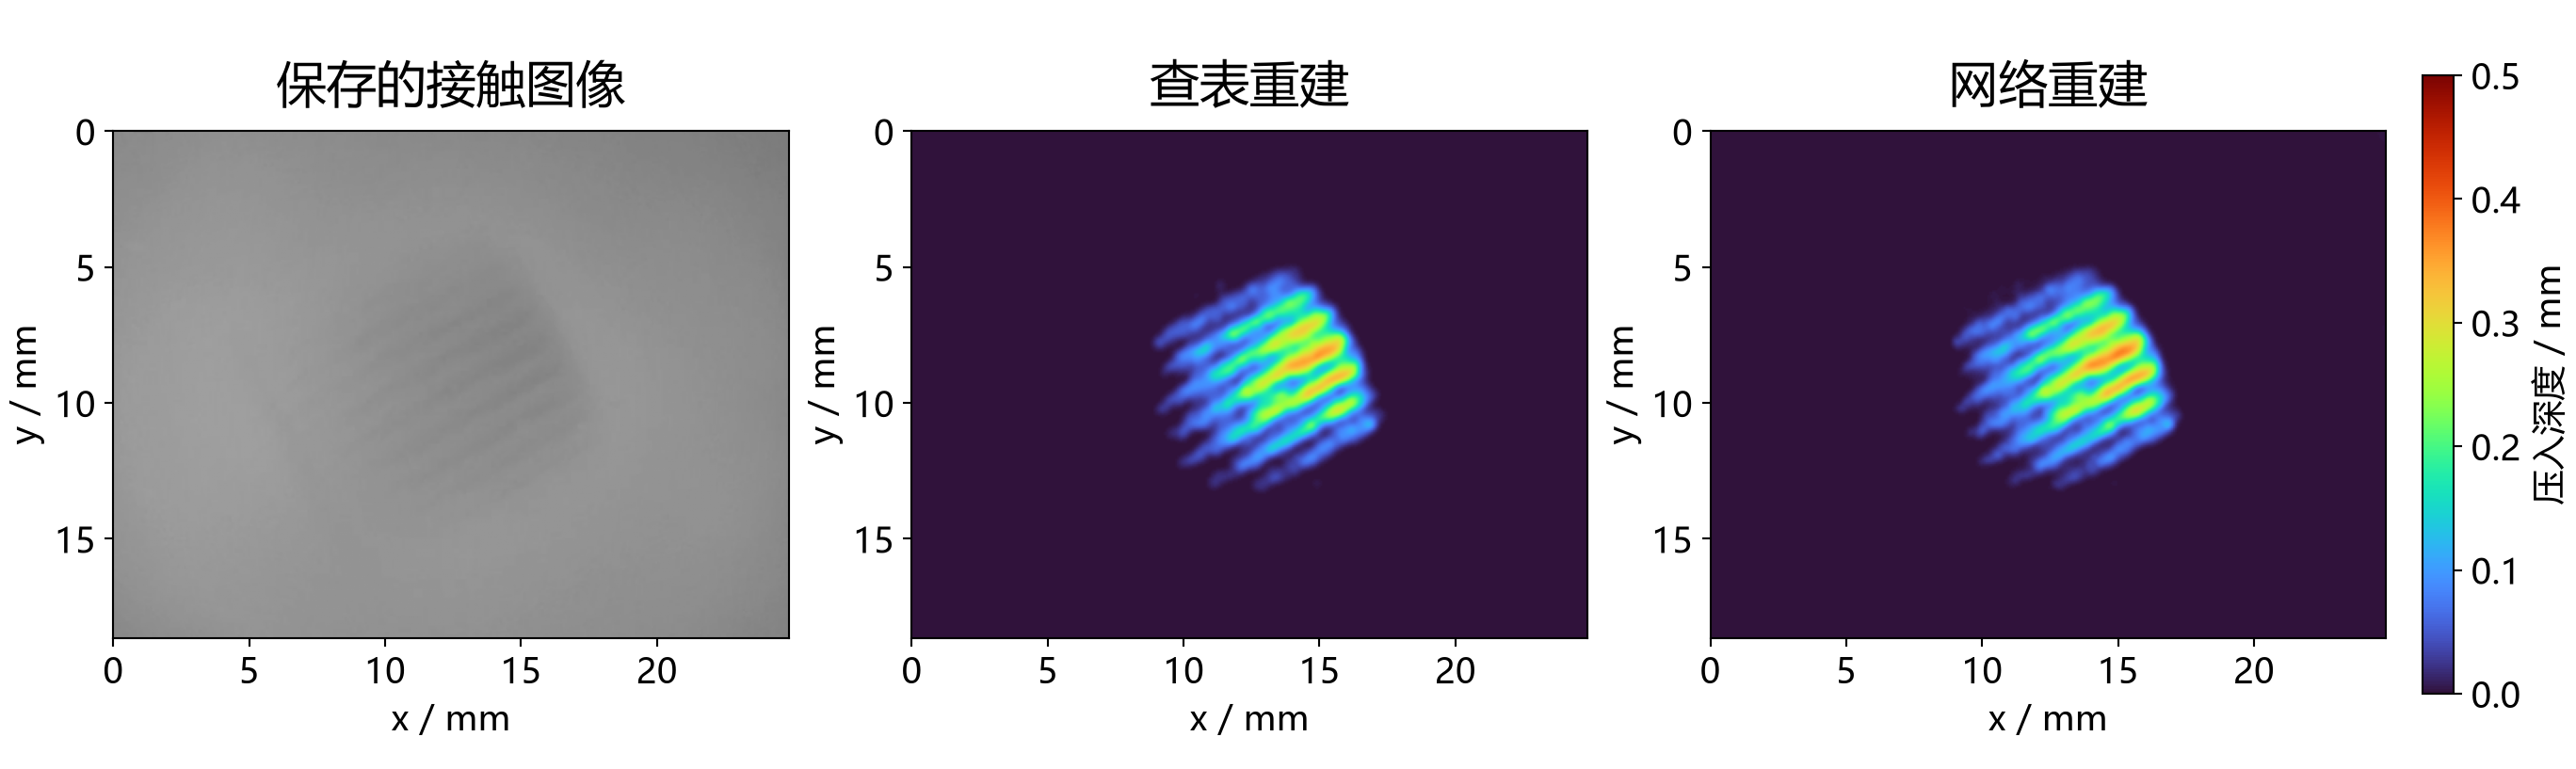
\includegraphics[width=\linewidth,height=36mm,keepaspectratio]{images/recorded_comparison.png}\par}
    {\centering\source{依据已有 NPZ 记录重绘；同一帧、同一 mm/pixel，两种高度图共用 0--0.5 mm 色标。}}
    \vspace{1mm}
    \begin{columns}[c,onlytextwidth]
      \column{.48\textwidth}
        \lead{训练与数据流程已贯通}\par
        {\small 3,000 帧合成数据／600 个接触组\par 按组划分：2,100／450／450 帧}
      \column{.48\textwidth}
        \lead{实时展示与保存已实现}\par
        {\small 相机输入、高度图、三维点云\par 支持 NPZ、PNG、PLY 导出与回放}
    \end{columns}
    \source{本页展示功能输出；没有独立真值，不据此判断两种方法的物理精度。}
    \note{【30 秒，累计 04:10】目前项目已经贯通数据、训练和展示流程。训练数据有三千帧，来自六百个合成接触组，按组划分以避免同一接触的相似帧跨集合。上面是仓库里保存的一帧输入及两条路径的重建结果，使用相同的毫米尺度和色标。程序还支持实时点云、结果导出和离线回放。接下来用真实接触展示这条处理链路。}
  \end{frame}

  % 09 / Recorded demonstration video, approximately 24 seconds.
  \begin{frame}[c]{演示视频：从按压到三维表面}
    \centering
    \embeddefensevideo{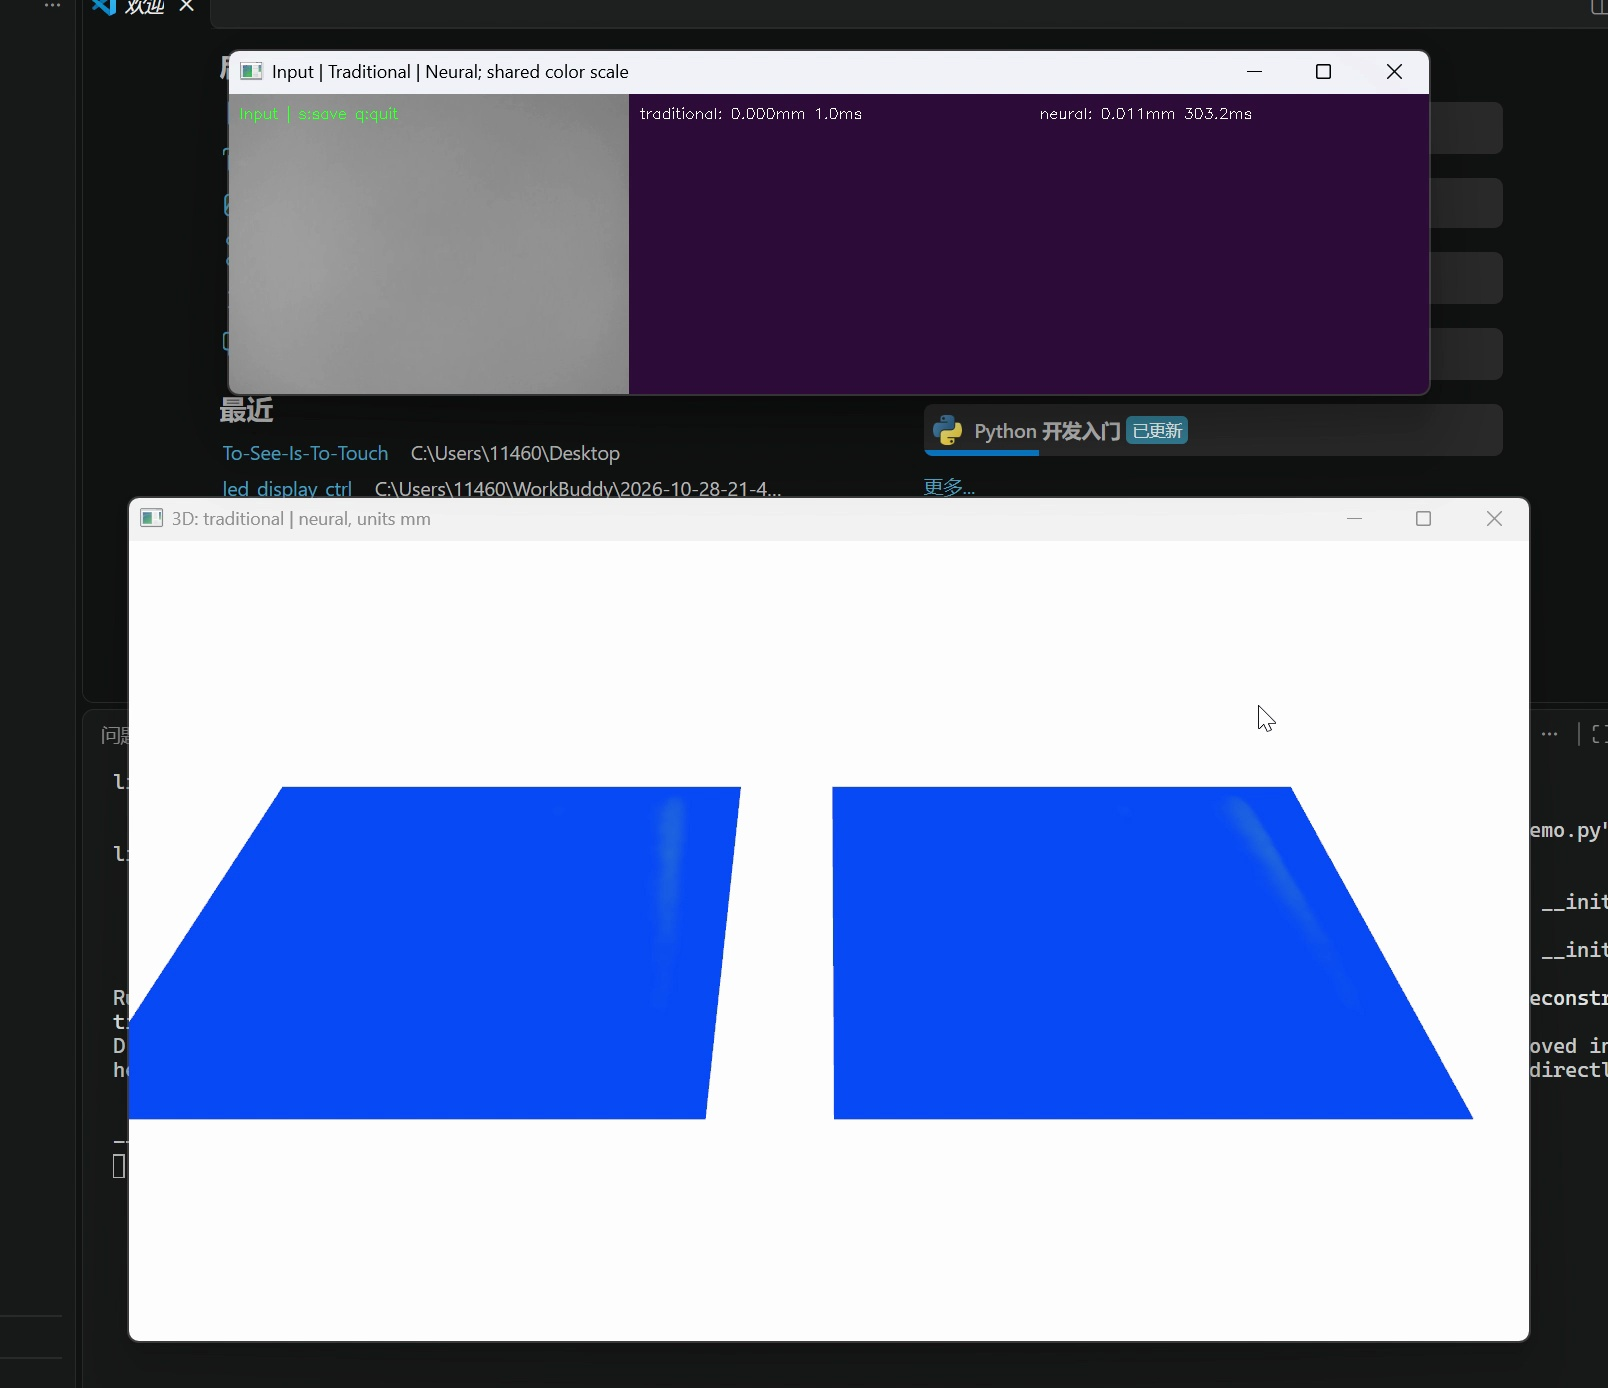
\includegraphics[height=53mm]{images/demo_video_poster.jpg}}{images/84a37282313403ba5020e64608b9926f_raw.mp4}
    \par\vspace{2mm}
    {\color{Teal}\bfseries 点击画面播放演示视频\par}
    \note{【演示视频，约 24 秒】点击画面播放已嵌入的传感器演示视频，结合输入画面、传统重建与网络重建结果进行讲解。视频原文件已包含在 PDF 内；播放需要支持 PDF 内嵌 H.264 视频的桌面阅读器。若当前阅读器无法播放，可直接打开 images/84a37282313403ba5020e64608b9926f_raw.mp4。播放结束后切换至后续研究方向。}
  \end{frame}

  % 10 / Closing remarks
  \begin{frame}[c]{后续研究方向}
    \relax
    {\centering
      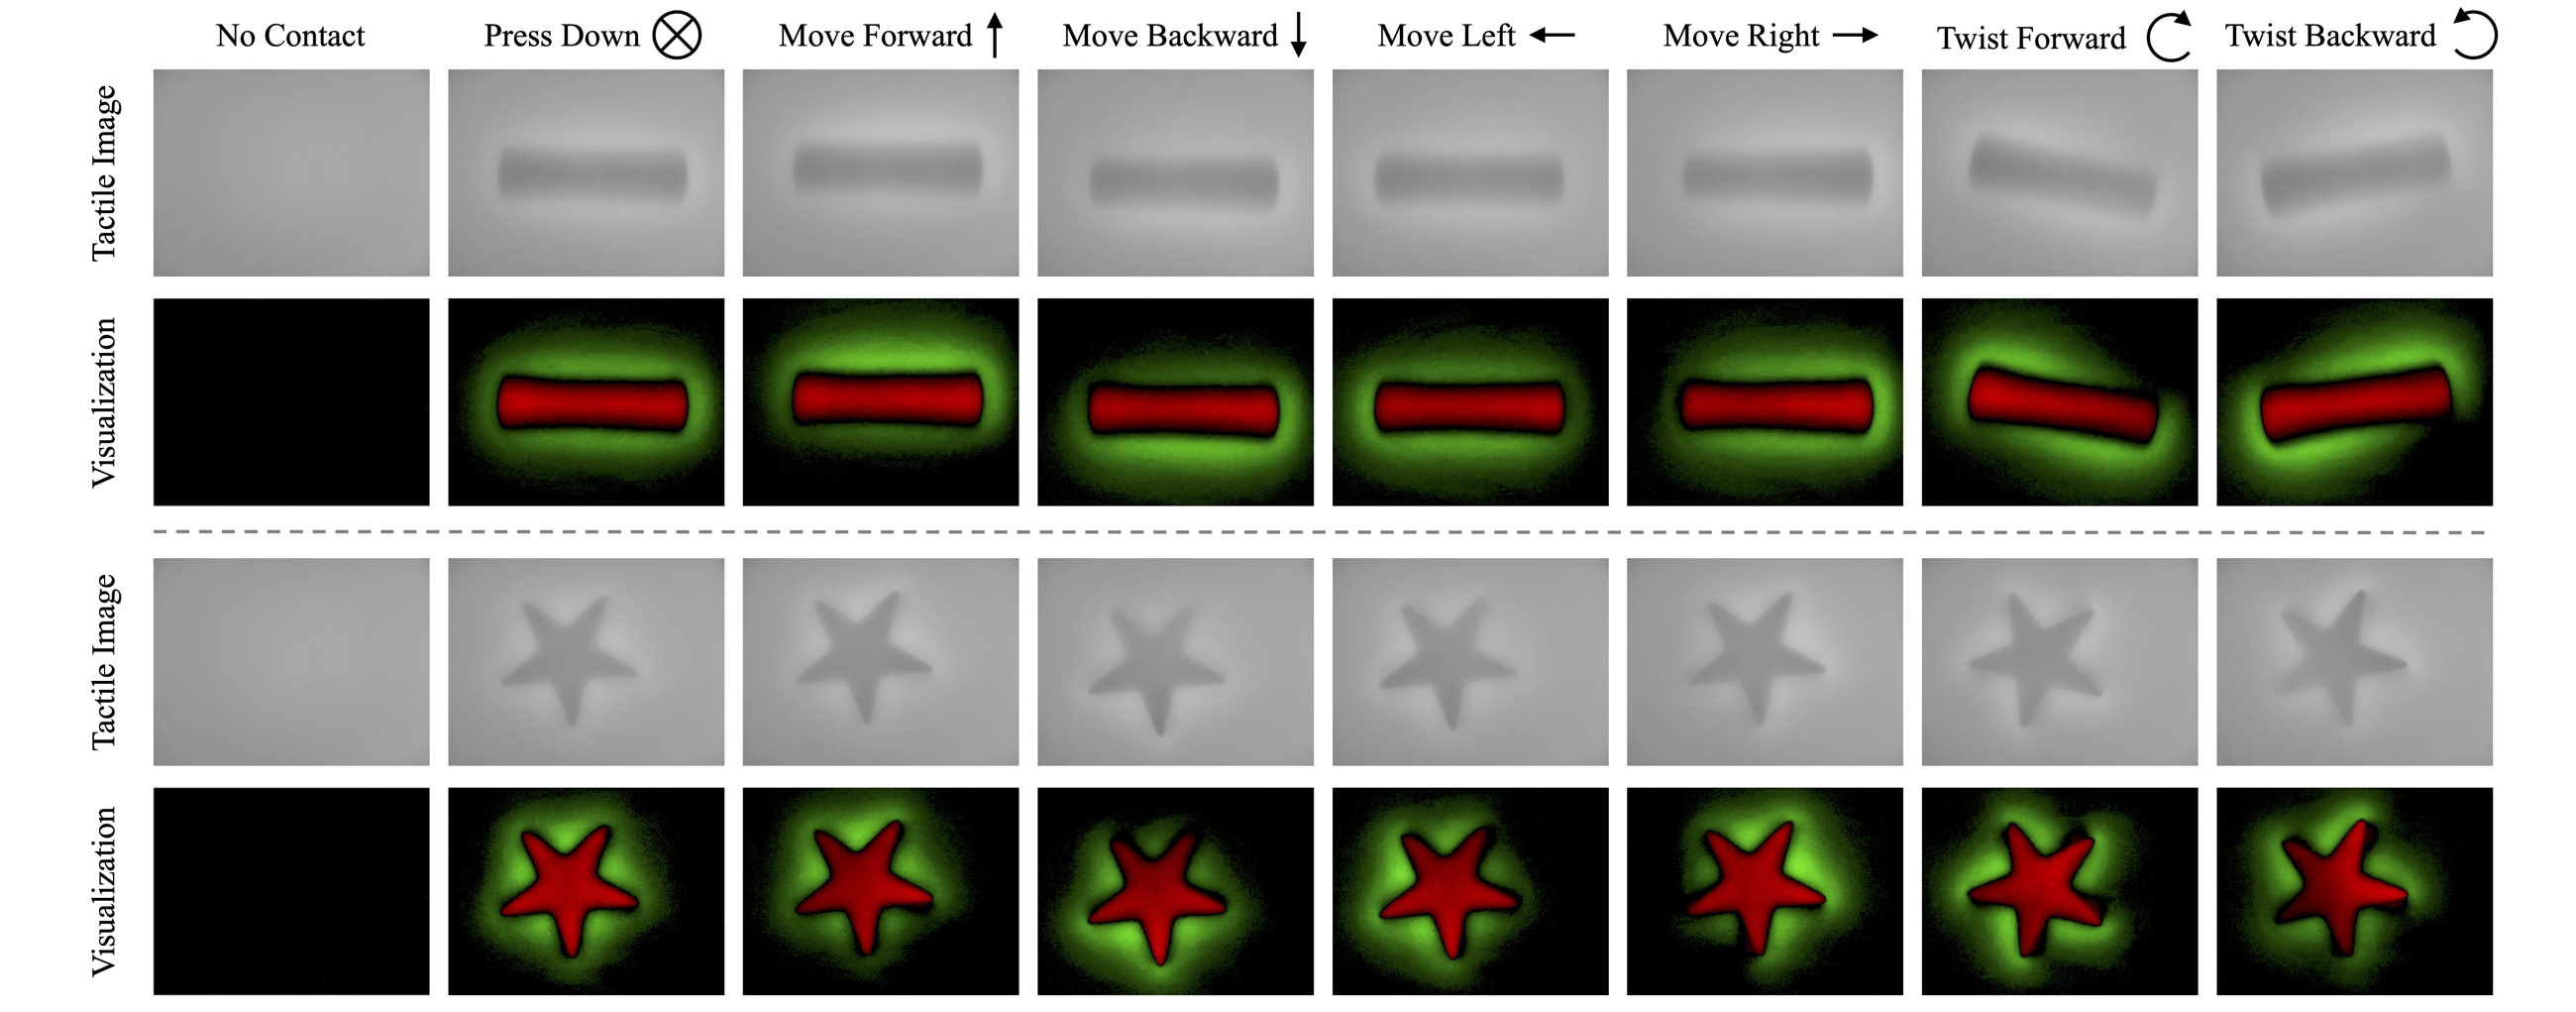
\includegraphics[width=\linewidth,height=34mm,keepaspectratio]{images/deformation_visualization.png}\par}
    \vspace{1mm}
    \begin{itemize}\setlength{\itemsep}{4pt}
      \item \lead{联合明暗信息}分析变暗接触区与周围变亮区域的形变。
      \item \lead{扩展运动感知}研究移动、扭转与亮区分布的对应关系。
      \item \lead{探索六维力估计}补充力学标定、真实数据与独立验证。
    \end{itemize}
    \source{当前已实现三维接触形状重建，尚未实现六维力估计。}
    \source{图示来源：9DTact 官网形变可视化示例，用户提供；非本项目采集或预测结果。}
    \note{【20 秒】后续我们希望联合利用变暗与变亮区域，分析接触区和周围凝胶的形变，进一步研究移动、扭转与亮区分布的关系。在此基础上探索六维力估计，并补充力学标定、真实数据和独立验证。目前项目已实现三维接触形状重建，尚未实现六维力估计。谢谢各位老师。}
  \end{frame}

\end{document}
